%%% Template originaly created by Karol Kozioł (mail@karol-koziol.net) and modified for ShareLaTeX use

\documentclass[a4paper,11pt]{article}

\usepackage[T1]{fontenc}
\usepackage[utf8]{inputenc}
\usepackage{graphicx}
\usepackage{xcolor}
 \usepackage{tgtermes}
\usepackage{listings}

 \usepackage[
 pdftitle={Math Assignment},
 pdfauthor={Joe Doe, Some University},
 colorlinks=true,linkcolor=blue,urlcolor=blue,citecolor=blue,bookmarks=true,
 bookmarksopenlevel=2]{hyperref}
\usepackage{amsmath,amssymb,amsthm,textcomp}
\usepackage{enumerate}
\usepackage{multicol}
\usepackage{tikz}

\usepackage{geometry}
\geometry{total={210mm,297mm},
left=25mm,right=25mm,%
bindingoffset=0mm, top=20mm,bottom=20mm}


\linespread{1.3}

\newcommand{\linia}{\rule{\linewidth}{0.5pt}}

% custom theorems if needed
\newtheoremstyle{mytheor}
    {1ex}{1ex}{\normalfont}{0pt}{\scshape}{.}{1ex}
    {{\thmname{#1 }}{\thmnumber{#2}}{\thmnote{ (#3)}}}

\theoremstyle{mytheor}
\newtheorem{defi}{Definition}
\usepackage[ruled, vlined, linesnumbered,lined,boxed,commentsnumbered]{algorithm2e}
\usepackage[parfill]{parskip}
\makeatletter

\setlength\parindent{0pt}
% custom footers and headers
\usepackage{fancyhdr,lastpage}


\newcommand{\myequ}[1]{\begin{align}\begin{split} #1 \end{split}\end{align}}


\begin{document}

\title{CSE 250B: Machine Learning}

\author{Sai Bi}

\date{\today}

\maketitle

\section*{Problem 1}
\subsection*{a}
For any $w_1$ and $w_2$, we have

\begin{align}
	\begin{split}
		L(w_1) + L(w_2) &= \sum_{i=1}^{n} ((y^{(i)} - w_1 \cdot x^{(i)})^2 + (y^{(i)} - w_2 \cdot x^{(i)})^2) \\
						& \geq  \sum_{i=1}^{N}\frac{(y^{(i)} -  w_1 \cdot x^{(i)} + y^{(i)} -  w_2 \cdot x^{(i)} )^2 }{2} \\
					& = 2 * \sum_{i=1}^{N} (y^{(i)} - \frac{w_1 + w_2}{2} x_{(i)})^2 \\
					& = 2 * L(\frac{w_1+w_2}{2})
	\end{split}
\end{align}

Hence $L(w)$ is a convex function.

\subsection*{b}\label{sec:1b}
Let $X$  be the data matrix where each row is a data point, and $Y$ be a column vector. Therefore we can rewrite $L(w)$
as $L(w) = (Y - Xw)^2$. The derivative of $L(w)$ is:
\myequ{
	L'(w) &= 2X^T(Xw-Y) 
}
Therefore the update rule should be 
\myequ{
	w_{t+1} &= w_t - 2\eta_{t} X^T (Xw-Y) 
}
where $\eta_{t}$ is the step size at step $t$.
\subsection*{c}
From Section~\ref{sec:1b} we know that $L'(w) = 2X^T(Xw-Y) $, and therefore $L''(w) = 2XX^T$, and therefore the update
rule should be
\myequ{
	w_{t+1} &= w_t - \eta_{t} L''(w)^{-1} L'(w)
}
where $\eta_{t}$ is the step size at step $t$.


\section*{Problem 2}
\subsection*{a}
\myequ{
	f(x_1) + f(x_2) -  2 * f(\frac{x_1 + x_2}{2}) & = x_1^T M x_1 + x_2^T M x_2 - 
		2 * (\frac{x_1+x_2}{2})^T M (\frac{x_1+x_2}{2}) \\
		& =	\frac{1}{2} (x_1^T M x_1 + x_2^T M x_2 - x_1^T M x_2 - x_2^T M x_1) \\
		& = \frac{1}{2} (x_1-x_2)^T M (x_1-x_2) \\
		& \geq 0 \text{ (since M is positive semi-definite)}
}	
Therefore $f(x_1) + f(x_2) \geq 2 f(\frac{x_1+x_2}{2})$, that is, $f(x)$ is convex.

\subsection*{b}
\myequ{
	f(x_1) + f(x_2) -  2 * f(\frac{x_1 + x_2}{2}) &=
		e^{u x_1} + e^{u x_2} - 2 * e^{u \frac{x_1+x_2}{2}} \\
		& \geq 2 \sqrt{e^{u x_1} e^{u x_2}} - 2 * e^{u \frac{x_1+x_2}{2}} \\
		& = 0
}
Therefore $f(x_1) + f(x_2) \geq 2 f(\frac{x_1+x_2}{2})$, that is, $f(x)$ is convex.

\subsection*{c}
\myequ{
	f(x_1) + f(x_2) & = \max\{g(x_1), h(x_1)\} + \max\{g(x_2) + h(x_2)\}	\\
		&\geq g(x_1) + g(x_2) \\
		&\geq 2 * g(\frac{x_1 + x_2}{2}) \\
	f(x_1) + f(x_2) & = \max\{g(x_1), h(x_1)\} + \max\{g(x_2) + h(x_2)\}	\\
		&\geq h(x_1) + h(x_2) \\
		&\geq 2 * h(\frac{x_1 + x_2}{2})	\\
	f(x_1) + f(x_2) & \geq  \max\{2 * g(\frac{x_1 + x_2}{2}), 2 * h(\frac{x_1 + x_2}{2})\}\\
					& = 2 f(\frac{x_1 + x_2}{2}) 
}
Therefore $f(x_1) + f(x_2) \geq 2 f(\frac{x_1+x_2}{2})$, that is, $f(x)$ is convex.

\section*{Problem 3}

\subsection*{b}
\begin{figure}[h]
	\centering{
		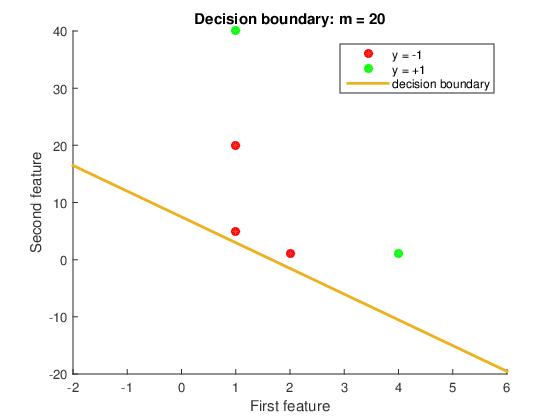
\includegraphics[width=0.45\textwidth]{./code/3b-20}
		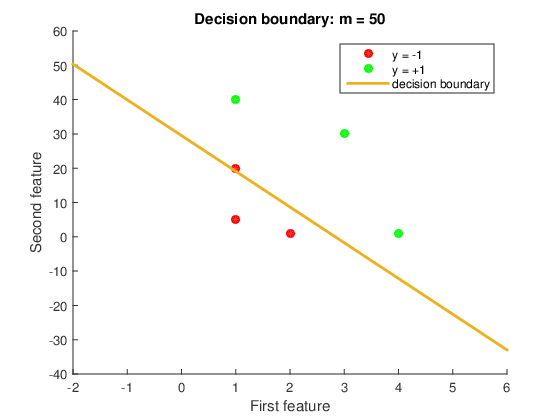
\includegraphics[width=0.45\textwidth]{./code/3b-50}	
		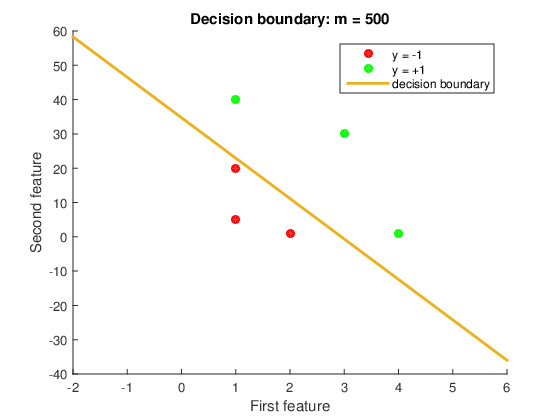
\includegraphics[width=0.45\textwidth]{./code/3b-500}	
		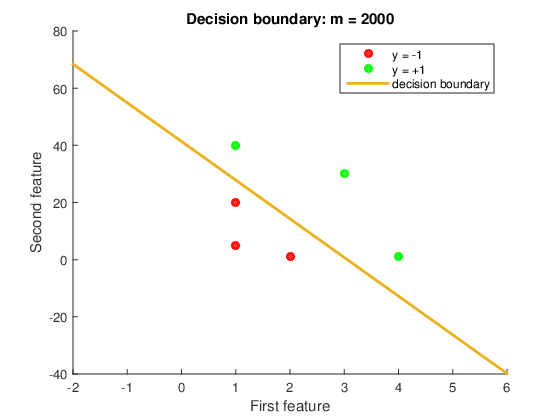
\includegraphics[width=0.45\textwidth]{./code/3b-2000}		
	}
	\caption{Problem 4-b}
\end{figure}

\subsection*{c}
The number of iterations needed for convergence \textbf{significantly increases} after scaling.


\subsection*{d}
\begin{figure}[h]
	\centering{
		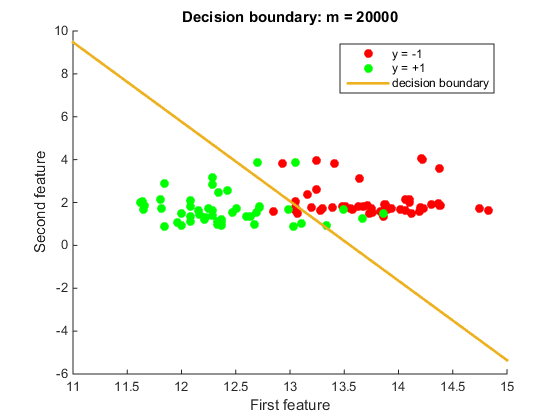
\includegraphics[width=0.7\textwidth]{./code/3d-20000}		
	}
	\caption{Problem 4-d}
\end{figure}
















\end{document}
